\documentclass[a4paper, 11pt]{article}

% Nécessaire
\usepackage[utf8]{inputenc}
\usepackage[T1]{fontenc}
\usepackage{lmodern}

% Biblio
\usepackage{natbib}
\bibliographystyle{abbrvnat}
\usepackage{hypernat}
\bibpunct{\textcolor{blue}{[}}{\textcolor{blue}{]}}{}{a}{\textcolor{blue}{,}}{;}

\usepackage[french]{babel}
\usepackage{amsmath, amsthm}
\usepackage{amsfonts,amssymb}

% Marge
\usepackage{geometry}
\geometry{margin={2.2cm ,2cm}}

% Figures, graphiques
\usepackage{graphicx}
\usepackage{epsfig}
\usepackage{caption}

% Surlignage
\usepackage{alltt}

\usepackage{xcolor}
\usepackage{soul}
\usepackage{color}
\usepackage{colortbl}

% Indicatrice
\usepackage{dsfont}

\usepackage{multirow}
\usepackage{eurosym}
\usepackage{extarrows}
\usepackage[colorlinks=true, citecolor=blue, linkcolor=.]{hyperref}

% Graphique
\usepackage{tikz}


% Titre
\title{Calibration du modèle en utlisant des inflorescences aux stades C/D/E}
\author{}
\date{}



\begin{document}
 \maketitle
 
 On utlise ici des dynamiques d'inflorescences simulées aux stades C, D et E en entrée du modèle. On fait cela car on pense que ce serait potentiellement les seuls stades qui pourraient être réellement attractifs pour les cécidomyies. En fin de saison, il y aurait alors une majorité d'inflorescences au stade F, ce qui engendrerait un manque de ressource pour les cécidomyies : cela pourrait alors être l'explication de la diminution finale des cécidomyies.
 
 \section{Inflorescences}
 
 Pour calculer le nombre d'inflorescences aux stades C/D/E à chaque date, on part des débourrements quotidiens simulés et on calcule les inflorescences vivantes en considérant qu'elles vivent toutes 16 jours --- les 16 jours correspondant à la durée théorique des stades C/D/E \citep{laurie}.
 Les dynamiques produites sont visibles sur la figure~\ref{titi}. Si l'on observe des phénomènes bizares (\emph{i.e.} le nombre d'inflos aux stades C/D/E dépasse parfois le nombre d'inflos attractives), on remarque une baisse conséquente du nombre d'inflos au stades C/D/E sur la fin, ce qu'on espérait.
 \begin{figure}[ht]
 \centering
 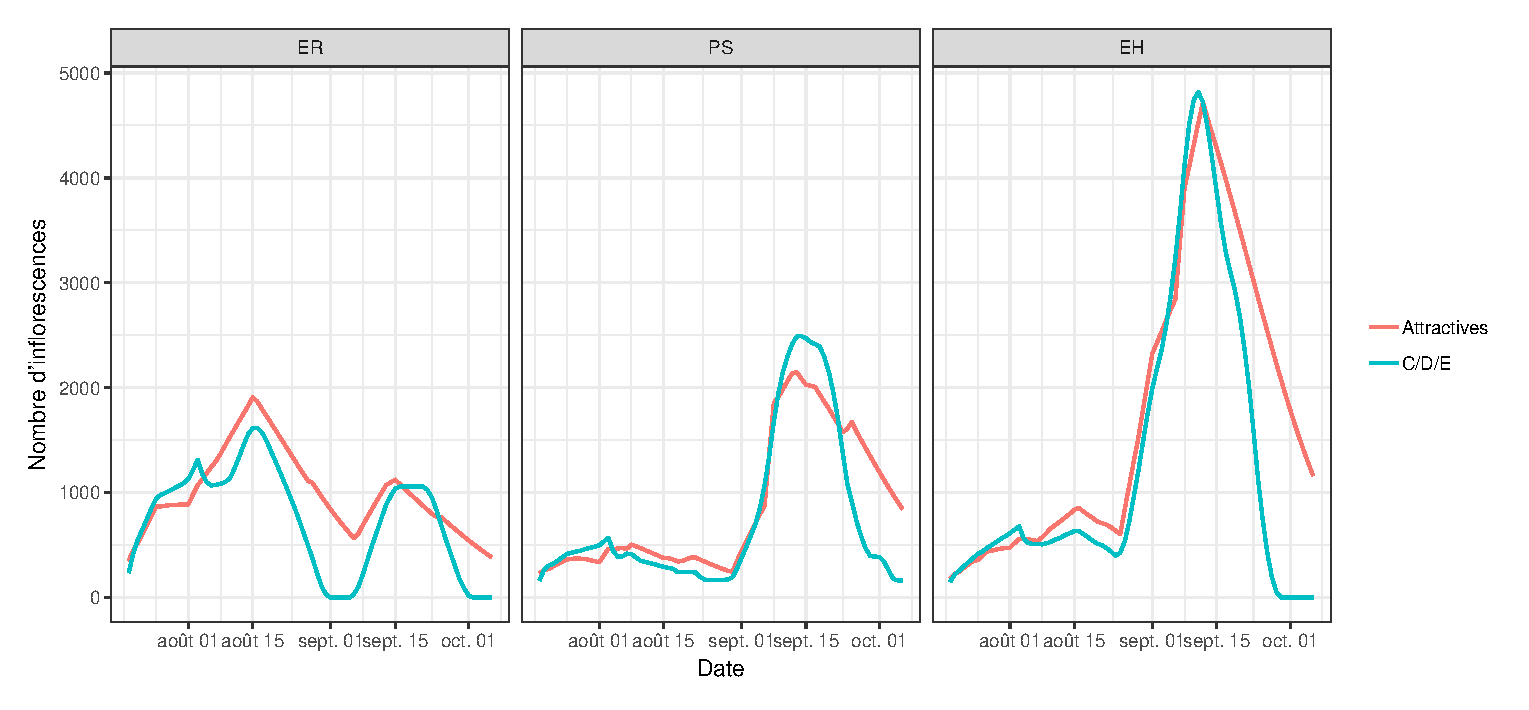
\epsfig{file = plots/attra_vs_cde.eps, scale = 0.65}
 \caption{Comparaison des dynamiques d'inflorescences. Les attractives sont celles utilisées d'habitude.}
 \label{titi}
 \end{figure}

 \section{Résultats}
 
 En calibrant le modèle (avec diapause) avec les inflorescences aux stades C/D/E en entrées, on peut trouver les paramètres suivants :
 \begin{center}
\begin{tabular}{llllll}
$\gamma$ & $p_m$ & $\mu_{\text{ER}}$ & $\mu_{\text{EH}}$ & $k$ & \texttt{stock}\\
0.020 & 0.094 & 0.989 & 0.709 & 0.232 & 5708
 \end{tabular}
 \end{center}

Les dynamiques associées sont visibles sur la figure \ref{tutu}.
 \begin{figure}[ht]
 \centering
 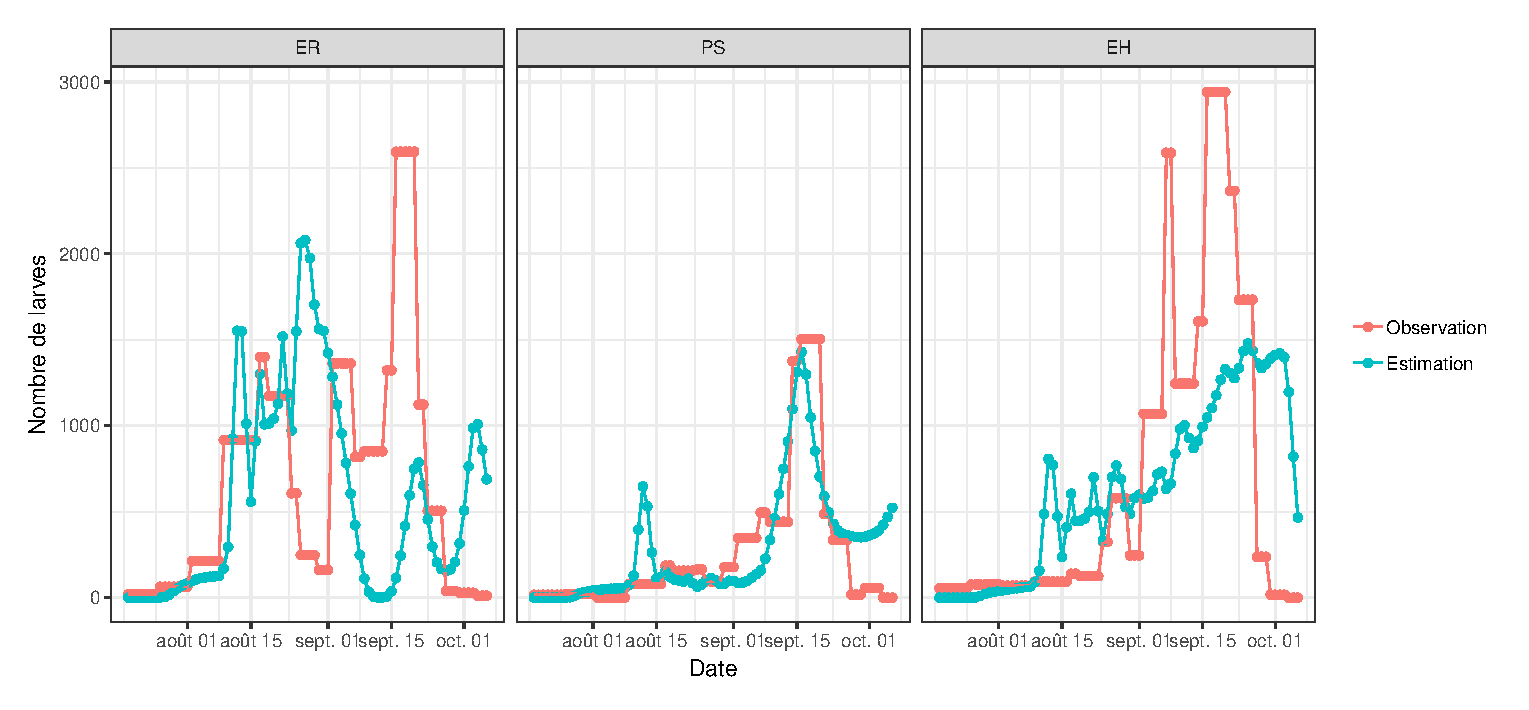
\epsfig{file = plots/larvesCDE.eps, scale = 0.65}
 \caption{Estimation avec les inflorescences aux stades C/D/E en entrées}
 \label{tutu}
 \end{figure}

 
 \vfill
 \bibliography{stadeCDE}
 
 
 
\end{document}


